\chapter{Network evolution}

\section{IoT}

The Cisco IoT System has six technology pillars: Network Connectivity, Fog computing, Security, Data analysis, Management and Automation, Application Enablement Platform.\\

The Cisco IoT network connectivity pillar identifies devices that can be used to provide IoT connectivity to many diverse industries and applications.\\

\textbf{Fog computing} is an IoT network model. It enables end devices to run applications \emph{locally} and make immediate decisions. This reduces the data burden on networks, as raw data does not need to be sent over network connections. It enhances resiliency by allowing IoT devices to operate when network connections are lost. It also enhances security by keeping sensitive data from being transported beyond the edge where it is needed.\\

The Cisco IoT security pillar offers scalable cybersecurity solutions:

\begin{itemize}
\item \textbf{Operational Technology (OT)} keeps power plants running and manages factory process lines
\item \textbf{IoT Network security} includes network and perimeter security devices (e.g. switch, router)
\item \textbf{IoT Physical security} enables surveillance in a wide variety of environments with Cisco Video Surveillance IP Cameras
\end{itemize}

The \textbf{Cisco IoT analytics} infrastructure consists of distributed network infrastructure components and IoT-specific, application programming interfaces (APIs).

\section{Cloud computing}

Cloud computing is a network model where servers and services are dispersed globally in distributed data centers. Cloud computing, with its “pay-as-you-go” model, allows organizations to treat computing and storage expenses more as a utility rather than investing in infrastructure. Capital expenditures are transformed into operating expenditures.\\

\subsection{Cloud service}

\begin{itemize}
\item \textbf{SaaS} (Software as a Service): The cloud provider is responsible for access to services, such as email, communication, and Office 365 that are delivered over the Internet. The user is only needs to provide their data.
\item \textbf{PaaS} (Platform as a Service): The cloud provider is responsible for access to the development tools and services used to deliver the applications.
\item \textbf{IaaS} (Infrastructure as a Service): The cloud provider is responsible for access to the network equipment, virtualized network services, and supporting network infrastructure.
\item \textbf{ITaaS} (IT support as a Service): cloud service providers provide IT support for each of the cloud computing services
\end{itemize} 

\subsection{Cloud model}

\begin{itemize}
\item \textbf{Public clouds:} Cloud-based applications and services offered in a public cloud are made available to the general population. Services may be \emph{free} or are offered on a \emph{pay-per-use} model, such as paying for online storage. The public cloud uses the Internet to provide services.

\item \textbf{Private clouds:} Cloud-based applications and services offered in a private cloud are intended for a specific organization or entity, such as the \emph{government}. A private cloud can be set up using the organization's private network, though this can be expensive to build and maintain. A private cloud can also be managed by an outside organization with strict access security.

\item \textbf{Hybrid clouds:} A hybrid cloud is made up of two or more clouds (example: part private, part public), where each part remains a distinctive object, but both are connected using a single architecture. Individuals on a hybrid cloud would be able to have degrees of access to various services based on user access rights.

\item \textbf{Community clouds:} A community cloud is created for exclusive use by a specific community. The differences between public clouds and community clouds are the functional needs that have been customized for the community. For example, healthcare organizations must remain compliant with policies and laws (e.g., HIPAA) that require special authentication and confidentiality.
\end{itemize}

\subsection{Cloud Computing, Data Center, Virtualization}

The terms ``data center'' and ``cloud computing'' are often incorrectly used. These are the correct definitions of data center and cloud computing:

\begin{itemize}
\item \textbf{Data center:} Typically a data storage and processing facility run by an in-house IT department or leased offsite.
\item \textbf{Cloud computing:} Typically an off-premise service that offers on-demand access to a shared pool of configurable computing resources. These resources can be rapidly provisioned and released with minimal management effort.
\end{itemize}

Cloud computing is possible because of data centers. A data center is a facility used to house computer systems and associated components. Cloud computing is a service provided by data centers. Cloud service providers use data centers to host their cloud services and cloud-based resources.\\

The terms ``cloud computing'' and ``virtualization'' are often used interchangeably; however, they mean different things. Virtualization is the foundation of cloud computing. Cloud computing separates the application from the hardware. Virtualization separates the OS from the hardware. 

\section{Virtualization}

Server virtualization takes advantage of idle resources and consolidates the number of required servers. This also allows for multiple operating systems to exist on a single hardware platform. Virtualization offers a variety of benefits:

\begin{itemize}
\item Reduced cost: Virtualization enables server consolidation, which requires fewer physical servers and devices. It also lowers the monthly power, cooling costs and reduces the amount of required floor space.

\item Easier prototyping

\item Fault tolerance, improved disaster recovery
\end{itemize}

The \textbf{hypervisor} is a program that adds an abstraction layer on top of the real physical hardware. The abstraction layer is used to create virtual machines which have access to all the hardware of the physical machine such as CPUs, memory, disk controllers, and NICs. Each of these virtual machines runs a complete and separate operating system. There are two types of hypervisor:

\begin{figure}[hbtp]
\caption{Two types of hypervisor}
\centering
\subfigure[Type 1]{ 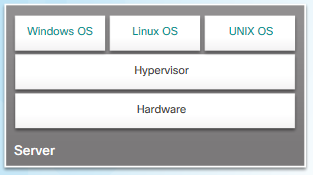
\includegraphics[ width=0.45\textwidth ]{pictures/HypervisorType1.PNG}\label{Type1} }
\subfigure[Type 2]{ 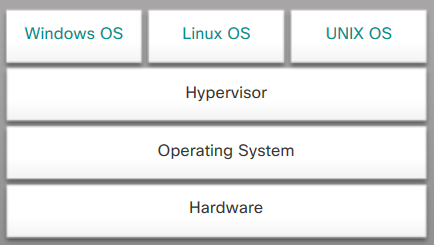
\includegraphics[ width=0.45\textwidth ]{pictures/HypervisorType2.PNG}\label{Type2} }
\end{figure}


\begin{itemize}
\item \textbf{Type 1:} the hypervisor is installed directly on the hardware. Then, instances of one or more OSes are installed on the hypervisor (Figure \ref{Type1}). Type 1 hypervisors have direct access to the hardware resources; therefore, they are more efficient than Type 2. This type of hypervisor requires a \emph{management console}.

\item \textbf{Type 2:} the hypervisor is installed on top of the existing OS (Windows, Mac OS, Linux, etc.). Then, one or more additional OS instances are installed on top of the hypervisor (Figure \ref{Type2}). A big advantage of Type 2 hypervisors is that management console software is not required. Type 2 hypervisors are very popular with consumers and for organizations experimenting with virtualization.
\end{itemize}

\textbf{Management console} is used to consolidate and turn on/off servers. It also provides recovery from hardware failure. If a server component fails, the management console automatically and seamlessly moves the VM to another server. \\

Some management consoles also allow \textbf{over allocation}. Over allocation is when multiple OS instances are installed, but their memory allocation exceeds the total amount of memory that a server has. For example, a server has 16 GB of RAM, but the administrator creates four OS instances with 10 GB of RAM allocated to each. This type of over allocation is a common practice because all four OS instances rarely require the full 10 GB of RAM at any one moment.

\section{SDN}

\subsection{Introduction}

A network device contains the following planes:

\begin{itemize}
\item \textbf{Control plane:} This is used to make forwarding decisions. The control plane contains Layer 2 and Layer 3 route forwarding mechanisms, such as routing protocol, neighbor tables and topology tables, routing tables, STP, and the ARP table.

\item \textbf{Data plane:} Also called the forwarding plane, this plane use information from the control plane to forward traffic flows. Information in the data plane is processed by a special data plane processor, such as a digital signal processor (DSP), without the CPU getting involved.
\end{itemize}

In a traditional router or switch architecture, the control plane and data plane functions occur in the same device. \textbf{Software defined networking (SDN)} is a network architecture that  virtualizes the control plane. It moves the control plane from each network device to a central network intelligence and policy-making entity called the \emph{SDN controller} or \emph{Network controller} (Figure \ref{SDNintro}). An example of Network controller is OpenDayLight platform. \\

\begin{figure}[hbtp]
\caption{Traditional and SDN architecture}\label{SDNintro}
\centering
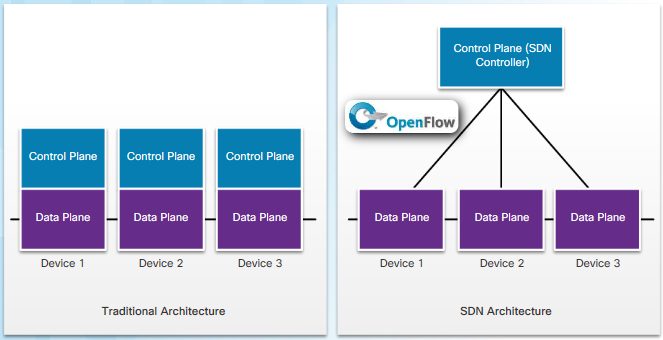
\includegraphics[ width=0.8\textwidth ]{pictures/SDNintro.PNG}
\end{figure}

\subsection{SDN controller}

The SDN controller enables network administrators to manage and dictate how the data plane of virtual switches and routers should handle network traffic. It orchestrates, mediates, and facilitates communication between applications and network elements.\\

\begin{figure}[hbtp]
\caption{SDN Framework}\label{SDNframework}
\centering
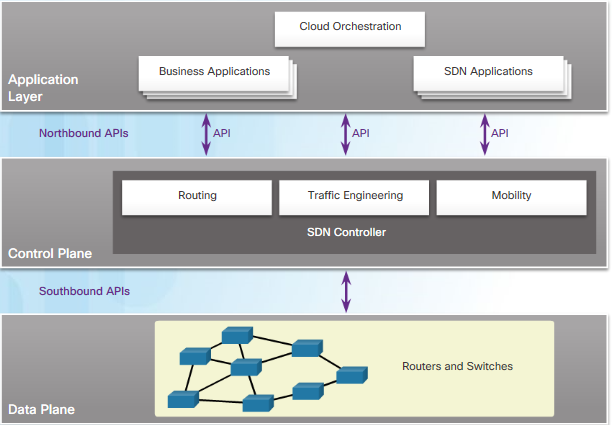
\includegraphics[scale=0.6]{pictures/SDNframework.PNG}
\end{figure}

Note the use of \textbf{API} (Application Programming Interfaces) within the SDN framework (Figure \ref{SDNframework}). An API is a set of standardized requests that define the proper way for an application to request services from another application. The SDN controller uses \emph{northbound} APIs to communicate with the applications. These APIs help network administrators shape traffic and deploy services. The SDN controller also uses southbound APIs to define the behavior of switches and routers. \\

\note Traffic in a modern data center is described as North-South (going between external data center users and the data center servers) and East-West (going between data center servers).\\

\subsection{Operation}

A \textbf{flow} is a sequence of packets traversing a network that share a set of header field values. For example, a flow could consist of all packets with the same source and destination IP addresses, or all packets with the same VLAN identifier.\\

\textbf{OpenFlow} protocol is a basic element of SDN which manages traffic between routers, switches, access points, and a controller. OpenFlow is the original southbound API. The Open Networking Foundation is responsible for maintaining the OpenFlow standard.\\

Each flow traveling through the network must first get permission from the SDN controller. If the controller allows a flow, it computes a route for the flow to take. Then, it adds an entry for that flow in each of the switches along the path by populating \emph{flow tables}. An SDN controller communicates with OpenFlow-compatible switches using the OpenFlow protocol. This protocol uses Transport Layer Security (TLS) to securely send control plane communications over the network.

\subsection{Types}

There are three types of SDN:

\begin{figure}[hbtp]
\caption{Three types of SDN}
\centering
\subfigure[Device-based]{ 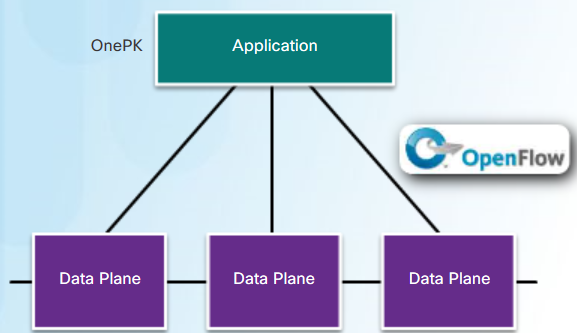
\includegraphics[width=0.45\textwidth]{pictures/DeviceBased.PNG}\label{DeviceBased}  }
\subfigure[Controller-based]{ 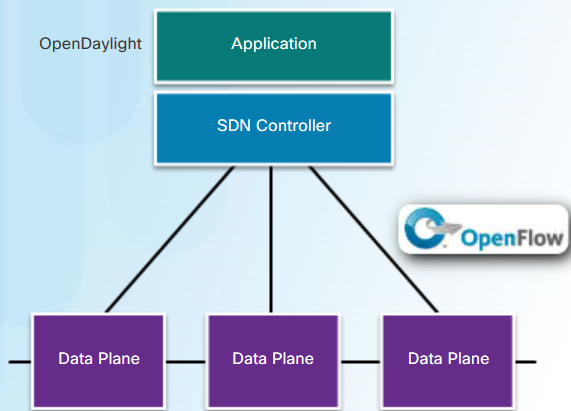
\includegraphics[width=0.45\textwidth]{pictures/ControllerBased.PNG}\label{ControllerBased} }
\subfigure[Policy-based]{ 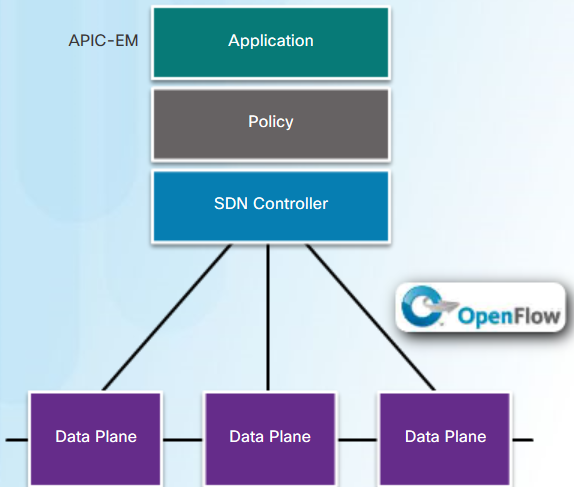
\includegraphics[width=0.6\textwidth]{pictures/PolicyBased.PNG}\label{PolicyBased} }
\end{figure}

\begin{itemize}
\item \textbf{Device-based SDN:} the devices are programmable by applications running on the device itself or on a server in the network, as shown in Figure \ref{DeviceBased}. \textbf{Cisco OnePK} is an example of a device-based SDN.

\item \textbf{Controller-based SDN} uses a centralized controller that has knowledge of all devices in the network, and manipulates traffic flows throughout the network, as shown in Figure \ref{ControllerBased}. The \textbf{OpenDaylight} and \textbf{Cisco Open SDN Controller} (commercial distribution of OpenDayLight) are examples of Controller-based SDN.

\item \textbf{Policy-based SDN} is similar to controller-based SDN where a centralized controller has a view of all devices in the network, as shown in Figure \ref{PolicyBased}. Policy-based SDN includes an additional Policy layer that operates at a higher level of abstraction. It uses built-in applications that automate advanced configuration tasks via a guided workflow and user-friendly GUI. No programming skills are required. \textbf{Cisco APIC-EM} is an example of Policy-based SDN.
\end{itemize}

\subsection{ACI}

\textbf{ACI} (Cisco Application Centric Infrastructure) is the Cisco's approach to SDN. It involves three main things: ANP, APIC, and programmable switches (Figure \ref{PolicyBased}):

\begin{itemize}
\item \textbf{Application Network Profile (ANP)} (the gray box in figure \ref{PolicyBased}) is a collection of end-point groups, their connections, and the policies that define those connections, such as VLANs, Web services, and applications.

\item \textbf{Application Policy Infrastructure Controller (APIC)} (blue box in figure \ref{PolicyBased}) is considered to be the brains of the ACI architecture. It manages and operates a scalable ACI clustered fabric. APIC is designed for programmability and centralized management. It translates application requirements  into network programming. The APIC is positioned between the APN and the ACI-enabled network infrastructure. 

\item \textbf{Cisco Nexus 9000 Series switches} (Figure \ref{SpineLeaf}) provide an application-aware switching fabric and work with an APIC to manage the virtual and physical network infrastructure.
\end{itemize}

\textbf{OpenStack} is an \emph{orchestration} platform that builds scalable cloud environments and provide IaaS solution. OpenStack is often used with Cisco ACI. Orchestration in networking is the process of automating the provisioning of network components such as servers, storage, switches, routers, and applications.

\begin{figure}[hbtp]
\caption{Spine-Leaf topology}\label{SpineLeaf}
\centering
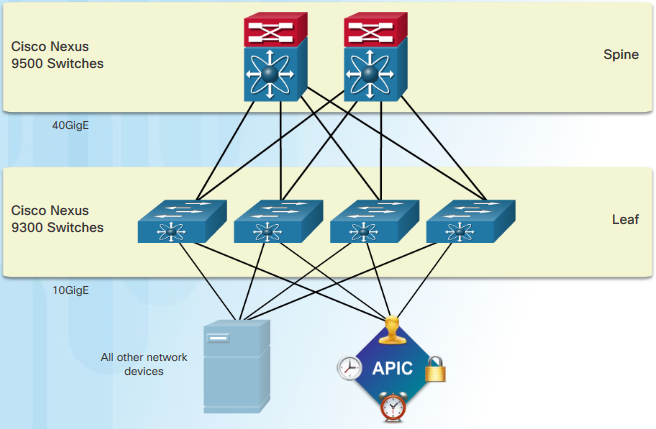
\includegraphics[ width=0.8\textwidth ]{pictures/SpineLeaf.PNG}
\end{figure}

The Cisco ACI fabric is composed of the APIC and the Cisco Nexus 9000 series switches using two-tier spine-leaf topology (Figure \ref{SpineLeaf}). The spine switches only attach to the leaf and core switches (not shown). In this two-tier topology, everything is one hop from everything else.\\

When compared to SDN, the APIC controller does not manipulate the data path directly. Instead, the APIC centralizes the policy definition and programs the leaf switches to forward traffic based on the defined policies.\\

\subsection{APIC-EM}

Cisco APIC-EM provides the following features:

\begin{itemize}
\item \textbf{Discovery:} populate the controller's device and host inventory database.

\item \textbf{Device Inventory:} collects detailed information from network devices (device name, device status, MAC address, etc.)

\item \textbf{Host Inventory:} - Collects detailed information from hosts (host name, user ID, MAC address, IPv4/IPv6 addresses, etc.)

\item \textbf{Topology:} graphical view of the network, auto-visualization of Layer 2 and 3 topologies on top of the physical topology

\item \textbf{Policy:} view and control policies across the entire network including QoS.

\item \textbf{Policy Analysis:} quickly identify ACLs in use and problem areas, enable ACL change management with easy identification of redundancy, conflicts and incorrect ordering of access control entries.
\end{itemize}

One of the most important features of the APIC-EM controller is the ability to manage policies across the entire network. APIC-EM ACL Analysis and Path Trace provide tools to allow the administrator to analyze and understand ACL policies and configurations: 

\begin{itemize}
\item \textbf{ACL Analysis} enables ACL \emph{inspection} and \emph{interrogation} across the entire network, exposing any problems and conflicts.

\item \textbf{ACL Path Trace} \emph{examines} specific ACLs on the path between two end nodes, displaying any potential issues.
\end{itemize}